\documentclass[12pt,a4paper]{article}
% \usepackage[UTF8]{ctex}
% \usepackage{minted}
\usepackage{fontspec}
\usepackage{titletoc}
\usepackage{xeCJK}
\usepackage{graphicx}
\usepackage{amsmath}
\usepackage{indentfirst} % 中文首段缩进
\usepackage{minted} % 代码块高亮渲染

% \setmainfont[Path=/usr/share/fonts/wenquanyi/wqy-microhei/]{wqy-microhei.ttc}
% \setCJKmainfont[Path=/usr/share/fonts/wenquanyi/wqy-microhei/]{wqy-microhei.ttc}
% \setmainfont[Path=/mnt/data/Fonts/NotoSans/]{NotoSans-Regular.ttf}
% \setCJKmainfont[Path=/mnt/data/Fonts/NotoSans/]{NotoSans-Regular.ttf}

\graphicspath{ {img/} }

\usepackage{xcolor}
\usepackage{hyperref}
\hypersetup{
    colorlinks=true,
    linkcolor=blue,
    urlcolor=red,
    linktoc=all
}
\definecolor{bg}{rgb}{0.95,0.95,0.95}
\newcommand{\incode}[1]{\mintinline[bgcolor=bg]{c}{#1}} % 定义行内代码渲染命令
\newcommand{\codefile}[1]{\inputminted[bgcolor=bg,linenos,tabsize=4]{verilog}{code/#1}} % 定义行内代码渲染命令
	
\renewcommand{\baselinestretch}{1.1} % 定义行间距
\parindent 24pt % 重新定义缩进长度
 
%%%%%%%%%%%%%%%%%%%%%%%%%%%%%%%%%%%%%%%%%%%%%%%%%%%%%%%%%%%%%%%%
%  lengths
%    下面的命令重定义页面边距,使其符合中文刊物习惯。
%%%%%%%%%%%%%%%%%%%%%%%%%%%%%%%%%%%%%%%%%%%%%%%%%%%%%%%%%%%%%%%%
\addtolength{\topmargin}{-54pt}
\setlength{\oddsidemargin}{-0.9cm}  % 3.17cm - 1 inch
\setlength{\evensidemargin}{\oddsidemargin}
\setlength{\textwidth}{17.00cm}
\setlength{\textheight}{25.50cm}    % 24.62

\title{实验三~流水线MIPS~CPU}
\author{张海斌\thanks{学号 17307130118}}
\begin{document}
\date{2019年5月}

\maketitle

\renewcommand\contentsname{目~录}
\tableofcontents

\section{概要}

流水线处理器与单周期处理器在结构上比较类似,但是流水线处理器通过时间上并行的方式提高CPU的吞吐率。最简单的流水线处理器的做法是将单周处理器分成取指令(Fetch)、译码(Decode)、执行(Execute)、存储器(Memory)、写回(Writeback)五个阶段,并在每两个阶段之间添加一个状态寄存器用来存储后续阶段运行所需的数据和控制信号。但是这样简单的流水线处理器在实际运行过程中会出现各种错误情况,比如写后读。所以为了让流水线处理器能正确运行,我们还需要增加冒险、预测分支等部份。

\section{功能展示}

LED[15]显示CPU时钟信号状态。SW[0]控制状态的清零,SW[1]控制CPU的运行和暂停,SW[3:2]控制七段数码管数据显示。当SW[3]为1时,八个七段数码管显示当前从指令内存(imem)中读取的32位指令。当SW[3]为0时,从左向右前两个七段数码管显示当前PC值,接着的两个数码管显示写入PC使能寄存器的值(只有当有使能信号的时候才会写入PC),最后四位七段数码管显示内存或寄存器中的值。此时,SW[9:4]提供需要查看的寄存器或内存的地址:当SW[2]为0时,以SW[8:4]的内容为寄存器地址,显示相应寄存器中的数据在右侧四个七段数码管上;当SW[2]为1时,以SW[9:4]的内容为内存地址,在相同的七段数码管上显示内存的数据。

\section{代码结构}

\begin{figure}[htbp]
	\centering
	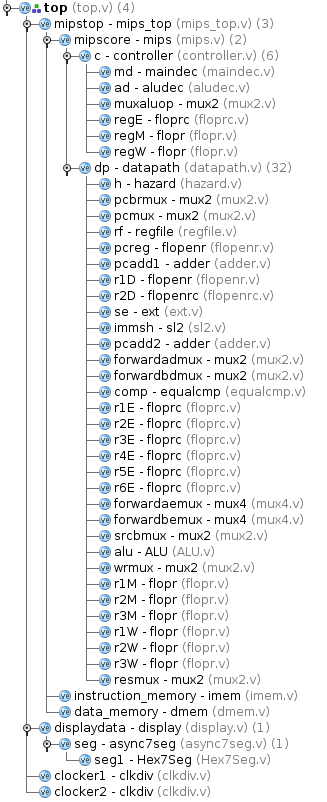
\includegraphics[width=0.25\textwidth]{struct}
	\caption{Verilog模块层次结构图}
	\label{fig:struct}
\end{figure}

Figure \ref{fig:struct} 展现了Verilog中各个模块的层次结构。\incode{top}是上板子的顶层文件,下面有两大模块\incode{mips_top}\ \incode{display}及两个时钟分频器 \incode{clkdiv}。\incode{mips_top}和\incode{display},分别为多周期处理器的顶层模块和负责处理板子显示的模块。在显示模块中包括了处理八个七段数码管连续显示的\incode{async7seg}模块,而它下含的\incode{Hex7Seg}则是将十六进制数转化为七段数码管上数字或字母显示的信号。\incode{mips_top}模块下主要有三个模块:\incode{mips}MIPS处理器核心、\incode{imem}指令内存和\incode{dmem}数据内存。在MIPS核心模块下分为两个模块:\incode{controller}控制器和\incode{datapath}数据通路。

\section{模块设计}

由于\incode{imem}与\incode{dmem}模块与单周期处理器完全相同,在报告中就不再赘述了。

\subsection{\incode{display}显示模块}

\begin{listing}[h]
	\definecolor{bg}{rgb}{0.95,0.95,0.95}
	\codefile{display.v}
	\caption{\incode{display}模块数据显示的选择}
	\label{code:display}
\end{listing}

在\incode{display}模块中,使用\incode{if}语句和\incode{case}语句来根据控制信号控制七段数码管的显示数据(相应代码见 Listing \ref{code:display})。七段数码管要显示的数据存储在\incode{Data[31:0]}中,并被提供给\incode{async7seg}模块用于数据显示。和之前的显示模块相同地,使用了两个时钟分频模块分别为CPU和七段数码管的显示提供时钟信号。

\subsection{\incode{controller}控制器模块}

\begin{listing}[htbp]
	\definecolor{bg}{rgb}{0.95,0.95,0.95}
	\codefile{controller.v}
	\caption{\incode{controller}模块阶段控制信号寄存器}
	\label{code:controller}
\end{listing}

\incode{controller}模块中,除了和单周期处理器相同的与控制信号生成相关的\incode{maindec}模块、\incode{aludec}模块以及一个二选一多路选择器外,还添加了存储执行 Execute, Memory, Writeback 阶段所需控制信号的三个寄存器。这些寄存器中只有 Execute 阶段对应的寄存器带有 Clear 清除控制信号。通过清除控制信号,可以清除 Execute 阶段寄存器中的数据,从而使这条指令在流向后续阶段时不会改变内存或寄存器的值,也就等价于\incode{nop}指令。这个清除控制信号在冲突模块中将会被使用到。另一方面,三个阶段控制信号寄存器中的数据也是像流水线般从前向后传递数据,而且由于每个阶段都使用了部份控制信号,后续阶段的寄存器中控制信号数目逐层递减。相关代码见 Listing \ref{code:controller} 。

\subsection{\incode{datapath}数据通路模块}

\begin{figure}[htbp]
	\centering
	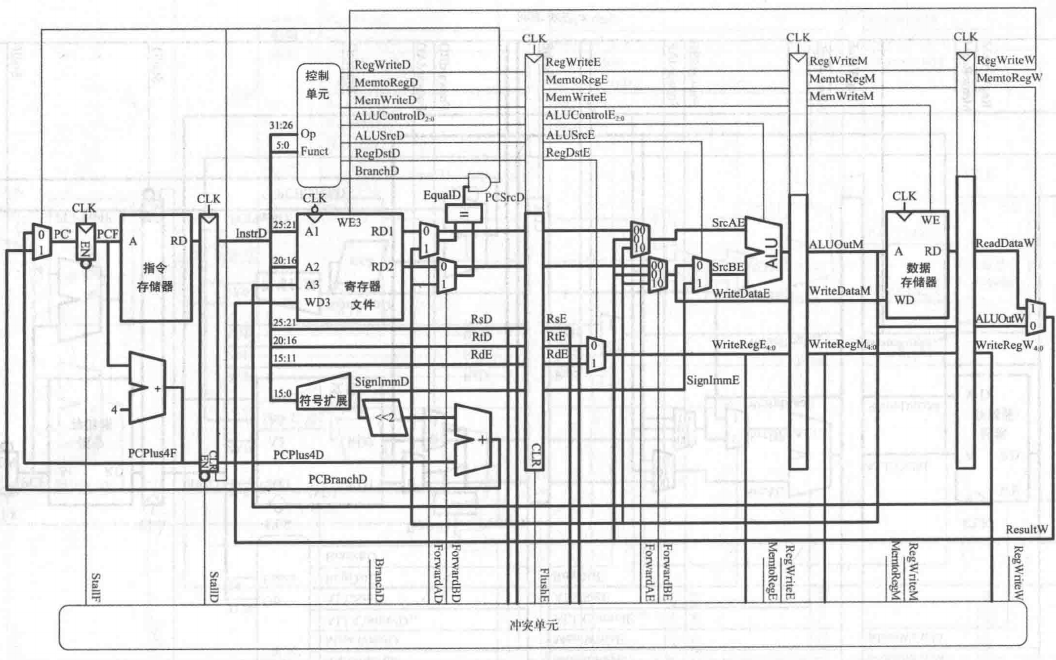
\includegraphics[width=0.9\textwidth]{datapath}
	\caption{流水线处理器结构图}
	\label{fig:datapath}
\end{figure}

在 Figure \ref{fig:datapath} 中完整画出了数据通路模块。相比于单周期处理器,数据通路中多了阶段数据寄存器、\incode{hazard}模块以及很多数据转发的线路。详细的冲突解决方法在 \ref{subsection} \incode{hazard}冲突模块 中进行解释。

我所实现的实际电路中,在\incode{PC'}的位置还有一个二选一多路选择器用来选择下一个PC是否为Jump指令对应的跳转地址。对于Branch指令,跳转判断发生在Decode阶段。默认预测为跳转不成功,即继续执行后续指令。如果Branch指令在Decode阶段跳转成功或者是Jump指令在Decode阶段,此时PC地址指向跳转指令的后一条指令处。在下一个时钟周期到来时,如果该PC对应的的指令写入Decode阶段数据寄存器,则它会被流水线错误地执行下去。所以我们要阻止其写入,即通过Decode阶段寄存器的Clear同步清除信号来控制错误指令不会写入其中。\incode{flushD}控制信号对应于Clear信号。

\subsection{\incode{hazard}冲突模块}\label{subsection}

\incode{hazard}模块主要用来解决流水线执行过程中可能遇到的执行错误的问题。下面就对各种错误情况进行解决。

对于写后读的情况,可以采用数据转发的方式解决,这种方法的好处是可以保证流水线的执行速度。在流水线CPU数据通路中,由于Decode阶段执行beq或bne指令需要使用通用寄存器以及Execute阶段ALU计算也需要通用寄存器中数据,所以这两个阶段读取通用寄存器的位置都需要多路选择器对数据进行选择。相应选择信号控制见 Listing \ref{code:forwardD}和 Listing \ref{code:forwardE} 。

\begin{listing}[htbp]
	\definecolor{bg}{rgb}{0.95,0.95,0.95}
	\codefile{forwardD.v}
	\caption{\incode{hazard}模块Decode阶段数据转发控制信号}
	\label{code:forwardD}
\end{listing}

\begin{listing}[htbp]
	\definecolor{bg}{rgb}{0.95,0.95,0.95}
	\codefile{forwardE.v}
	\caption{\incode{hazard}模块Execute阶段数据转发控制信号}
	\label{code:forwardE}
\end{listing}

首先我们讨论Decode阶段执行Branch指令时的转发问题。Writeback阶段如果有需要写回到寄存器中的数据,那么它会在本周期中的时钟下降沿写入,之后如果寄存器文件恰好读这个寄存器,那就会读出一个正确的结果,这样就不需要将Writeback阶段数据转发到Decode阶段,但我们仍需处理Execute阶段和Memory阶段的寄存器写入数据。如果Memory阶段执行的指令要写入我们在Decode阶段需要读取的寄存器而且Decode阶段正在执行Branch指令,我们就通过数据转发传输正确的数据到Decode阶段。这对Memory阶段不需要读取内存时是正确的,但如果是从内存中获取数据写入寄存器中,就无法正常转发了,这就需要通过stall解决,即暂停Fetch和Decode阶段执行,让Execute及后续阶段继续执行,同时在下一周期将Execute阶段数据和控制寄存器清零。这样在下一时钟周期内,转发的数据会在时钟下降沿写入寄存器文件,从而在Decode阶段获得正确的数据。对于Execute阶段执行指令要写入Decode阶段Branch指令读取的寄存器的情况,我们也通过stall的方式解决。这样,在下一周期时,问题就变成了转发Memory阶段的寄存器数据。stall控制信号代码见 Listing \ref{code:stall} 。

\begin{listing}[htbp]
	\definecolor{bg}{rgb}{0.95,0.95,0.95}
	\codefile{stall.v}
	\caption{\incode{hazard}模块stall信号}
	\label{code:stall}
\end{listing}

接着我们来讨论转发到Execute阶段的问题。因为Execute阶段使用的数据是在上一个周期的寄存器数据,且Writeback阶段更新的寄存器数据无法改变Execute阶段数据寄存器中的数据,所以我们需要通过数据转发将Writeback阶段更新的寄存器数据传递到Execute阶段。同样,Memory阶段对应执行的指令对寄存器的数据更新也应当转发到Execute阶段。Memory阶段指令有两种情况:一种是无需从数据内存中获得数据,此时直接转发即可;另一种是\incode{lw}指令,需要从数据内存中获取数据然后写入寄存器,这种情况只能让Execute阶段暂停一个周期,等其读出内存数据再进行转发,这也就相当与从Writeback阶段转发。为了简化电路,我们对于这种情况,即\incode{lw}指令写入寄存器后,后一条指令又读取同一个寄存器的情况,在后一条指令处于Decode阶段的时候让其暂停一个周期,这与让它在Execute阶段暂停一个周期的效果是等价的。判断这种情况的发生是 Listing \ref{code:stall} 中\incode{lwstallD}控制信号的作用。

\section{仿真结果}

\begin{figure}[htbp]
	\centering
	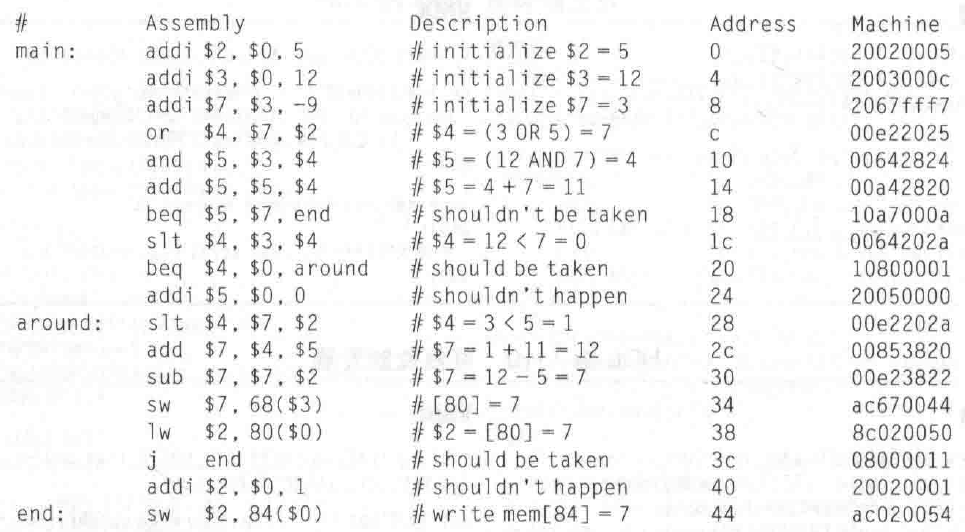
\includegraphics[width=0.75\textwidth]{code}
	\caption{测试代码}
	\label{fig:code}
\end{figure}

Figure \ref{fig:code}是测试使用的代码。Figure \ref{fig:sim1}和Figure \ref{fig:sim2}是流水线CPU仿真结果。值得注意的是\incode{PC}只是代表当前周期内\incode{PC}寄存器中的数据,也意味着当前周期内Fetch阶段从指令内存的\incode{PC}位置读取指令,但在后续阶段中是否真正执行这条指令尚不确定,因为Decode阶段数据寄存器可能会受Clear信号控制从而被清除掉。

内存的写入与读出即\incode{sw}与\incode{lw}指令经过验证是正确的。

\begin{figure}[htbp]
	\centering
	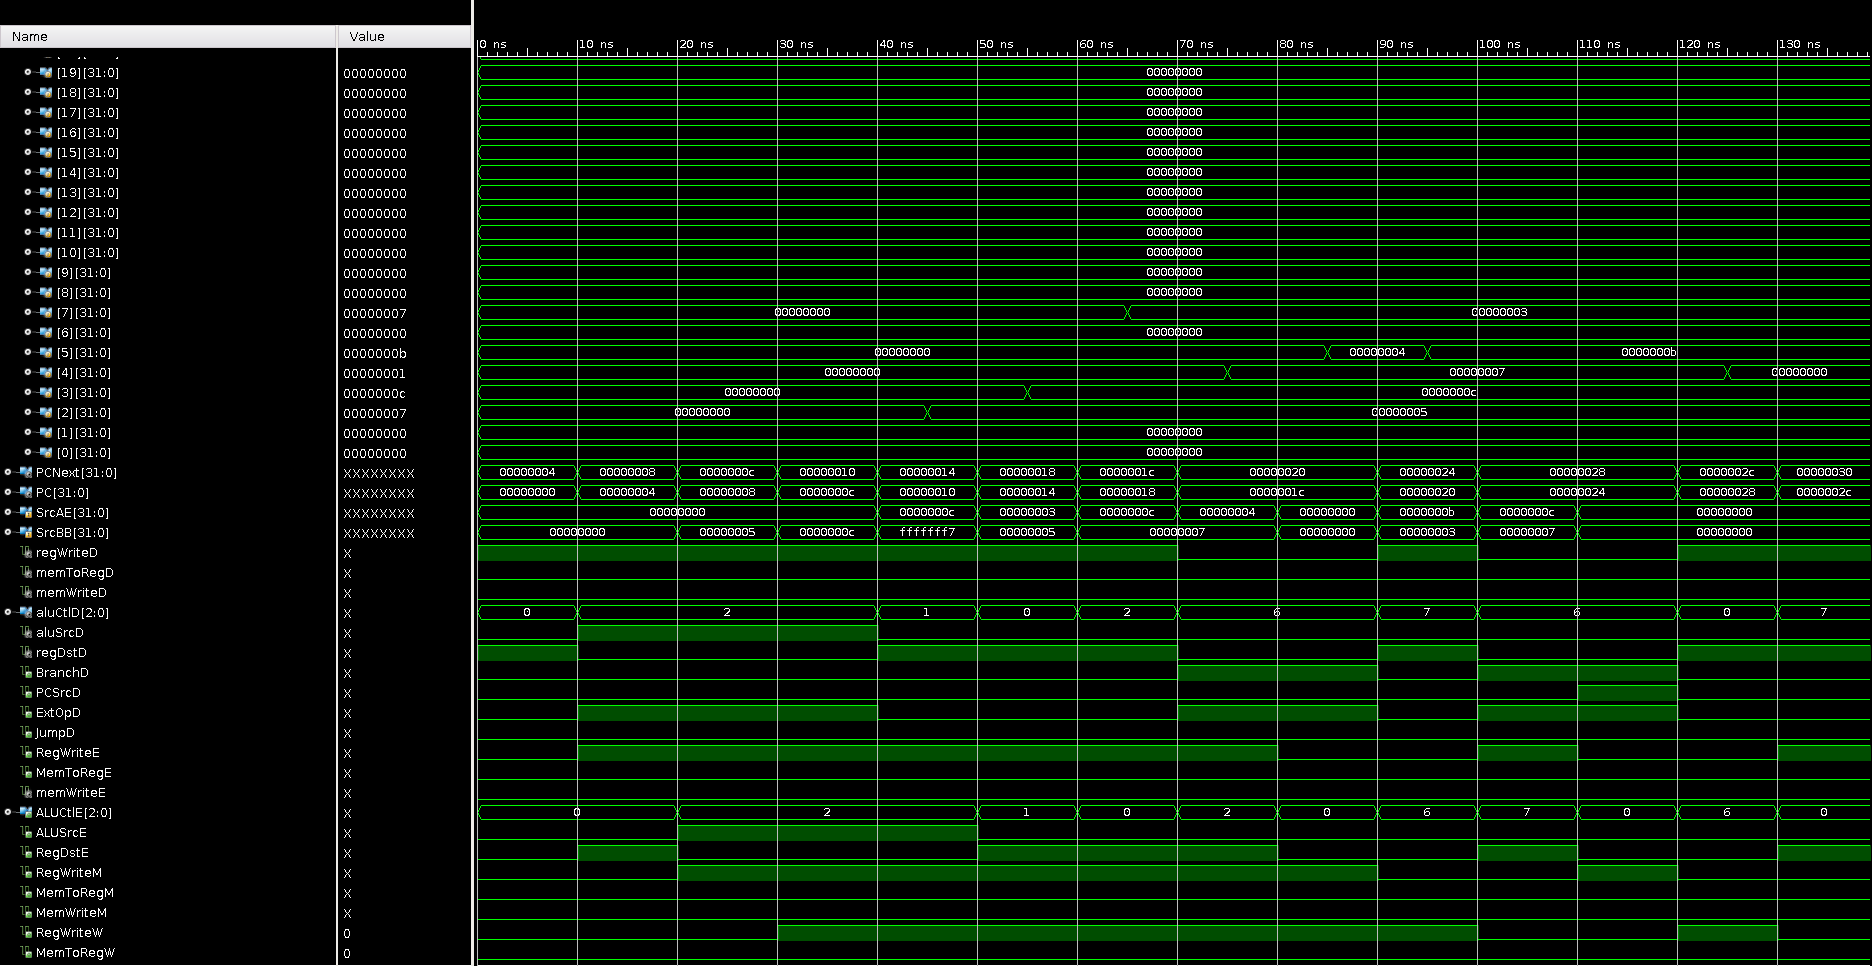
\includegraphics[width=\textwidth]{sim1}
	\caption{仿真测试图1}
	\label{fig:sim1}
\end{figure}

\begin{figure}[htbp]
	\centering
	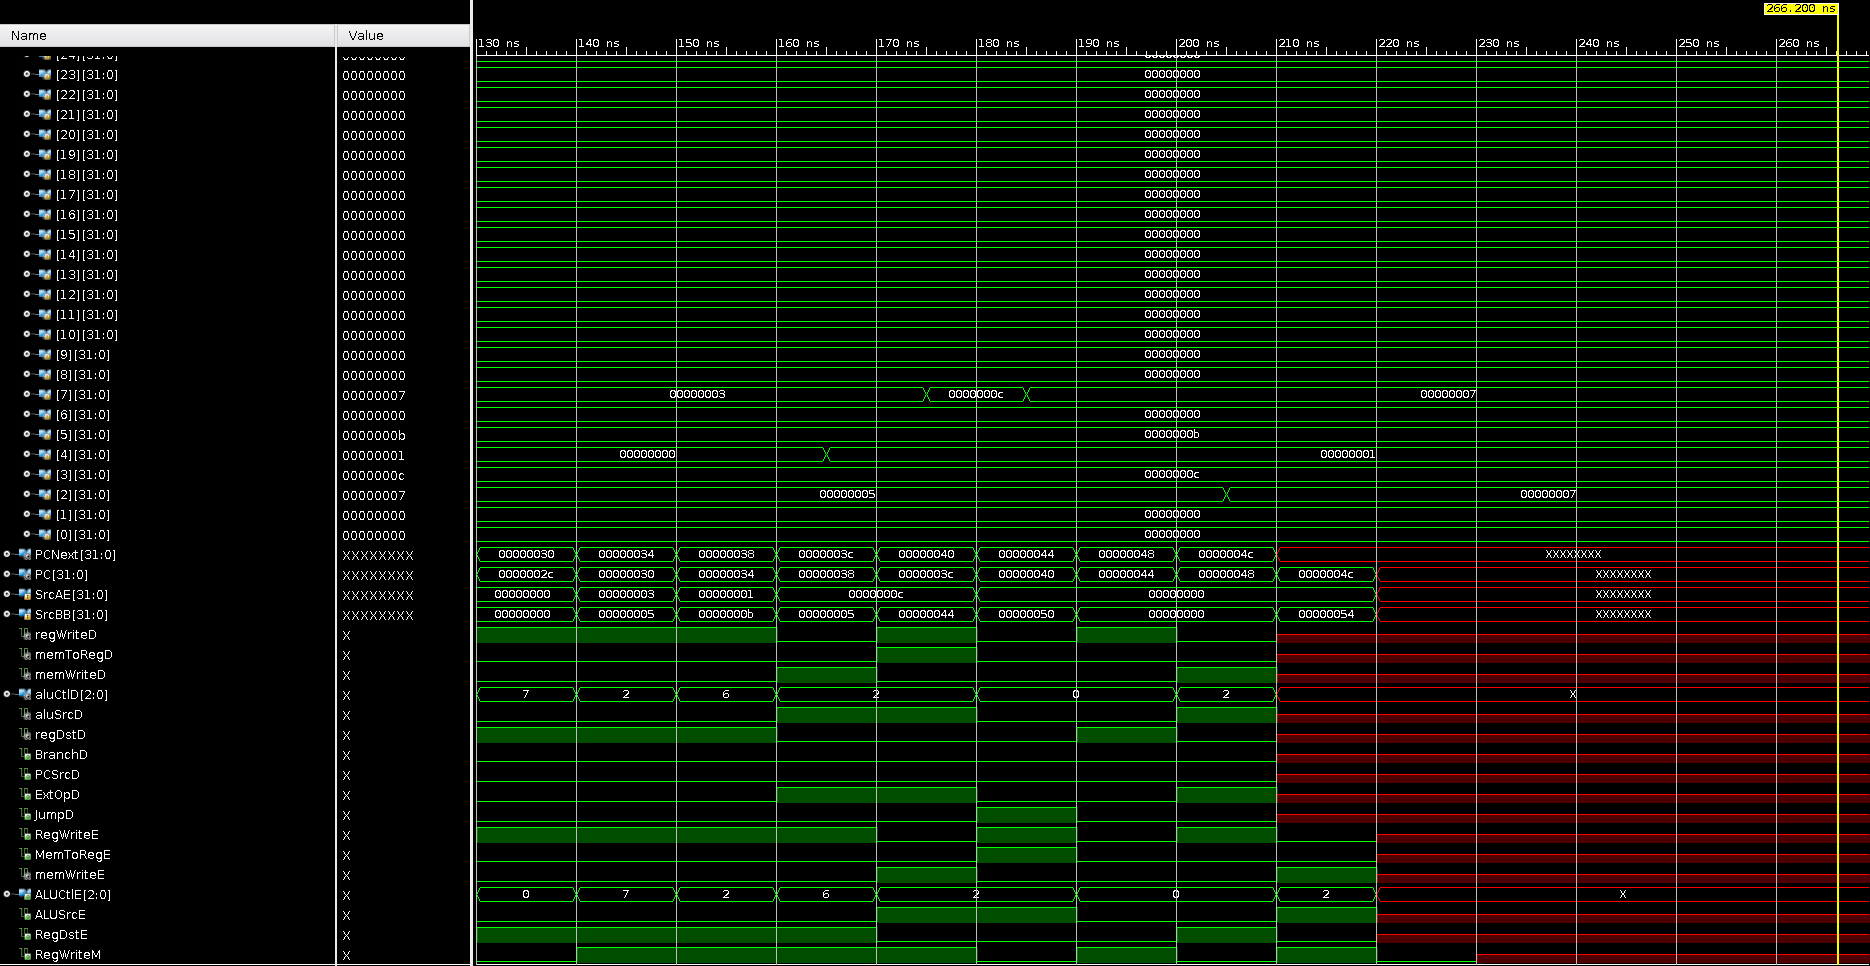
\includegraphics[width=\textwidth]{sim2}
	\caption{仿真测试图2}
	\label{fig:sim2}
\end{figure}

\end{document}
